\documentclass{article}
\usepackage{amsmath}
\usepackage{amssymb}
\usepackage{tikz}
\usetikzlibrary{arrows.meta, decorations.pathreplacing}
\usetikzlibrary{positioning}

\begin{document}

\begin{align*}
    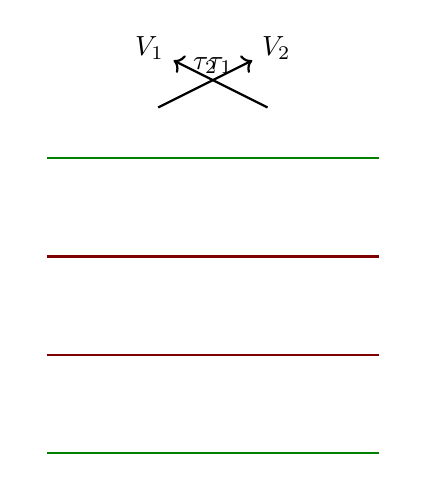
\begin{tikzpicture}[scale=0.75]
        \node (v1) at (-2,0) {$V_{1}$};
        \node (v2) [right=of v1] {$V_{2}$};
        
        % Nodes for V1
        \node (u1) [below left = 1cm and 1cm of v1] {};
        \node (u2) [below = 1cm of u1] {};
        \node (u3) [below = 1cm of u2] {};
        \node (u4) [below = 1cm of u3] {};
        
        % Nodes for V2
        \node (w1) [below right = 1cm and 1cm of v2] {};
        \node (w2) [below = 1cm of w1] {};
        \node (w3) [below = 1cm of w2] {};
        \node (w4) [below = 1cm of w3] {};
        
        % Draw edges
        \draw[green!50!black, thick] (u1) -- (w1);
        \draw[red!50!black, thick] (u2) -- (w2);
        \draw[red!50!black, thick] (u3) -- (w3);
        \draw[green!50!black, thick] (u4) -- (w4);
        
        % Arrows for V1 ordering
        \draw[<-,thick] (v1) -- ++(2,-1) node[midway,above] {$\tau_1$};
        
        % Arrows for V2 ordering
        \draw[<-,thick] (v2) -- ++(-2,-1) node[midway,above] {$\tau_2$};
    \end{tikzpicture} & \qquad
    \begin{tikzpicture}[scale=0.75]
        \node (v1) at (2,0) {$\sigma$};
        
        % Nodes for V2
        \node (w1) at (0,0) {};
        \node (w2) [below = 1cm of w1] {};
        \node (w3) [below = 1cm of w2] {};
        \node (w4) [below = 1cm of w3] {};
        
        % Draw edges
        \foreach \i in {1,...,4} {
            \node[circle,fill,inner sep=2pt,label={45:\i}] (\i) at (w\i) {};
        }
        
        \draw[->,thick] (v1) -- ++(3,0);
        \draw[<-,thick] (v1) -- ++(0,-2);
        
        % Draw lines
        \foreach \i in {1,...,4} {
            \pgfmathtruncatemacro{\j}{mod(\i+2,5)}
            \pgfmathtruncatemacro{\k}{mod(\i+3,5)}
            \draw[thick] (\i) -- (\j);
            \draw[thick] (\i) -- (\k);
        }
        
        % Arrows for V2 ordering
        \draw[<-,thick] (v1) -- ++(-3,-1) node[midway,above] {$\sigma$};
    \end{tikzpicture}
\end{align*}

\end{document}